\section{Model Design}

In this section, we will first introduce popular deep learning models used as baselines of our garbage dataset.

\subsection{Baselines}

We used three model architectures as our baseline of the dataset: VGGNet\cite{vgg2014}, ResNet\cite{resnet2016} and DenseNet\cite{densenet2017}. We also try the AlexNet\cite{alexnet} and SquezzeNet\cite{squeezenet2016}, but the training did not converge maybe due to the representation capacity. So we exclude these two models from our baseline list.

\subsubsection{VGGNet}

VGGNet is a Convolutional Neural Network architecture proposed by Karen Simonyan and Andrew Zisserman from the University of Oxford in 2014\cite{vgg2014}. This model mainly focuses on the effect of the convolutional neural network depth on its accuracy. This model won the 2014 ImageNet Large Scale Visual Recognition Competition, achieving an top5 accuracy of 92.9\% and top1 accuracy of 75.6\%. The architecture of VGGNet is shown in Figure \ref{fig:vgg}. VGGNet is composed of a stack of convolutional layers and 3 fully connected layers. Images directly passed through the model and the output is an 1000 dimensional vector to predict 1000 labels.
\begin{figure}[ht]
	\centering
	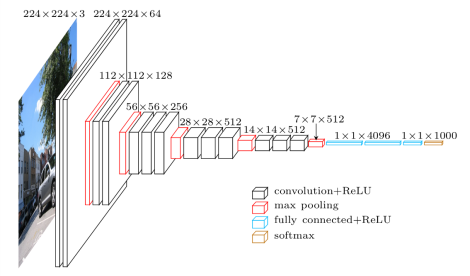
\includegraphics[scale=1.]{figs/vgg16.png}
	\caption{Architechture of VGG16\cite{vgg_arch}}
	\label{fig:vgg}
\end{figure}

The depth of VGGNet can vary by adjusting the number of convolutional layers. The model shown in Figure \ref{fig:vgg} is VGG16 composed of 13 convolutional layers and 3 fully connected layers, which add up to 16. Other popular VGG variants include VGG13 and VGG19. Batch normalization can also be added behind each convolutional layer to standardizes the inputs to a layer for each mini-batch. In the experiment, we test both classical and batch normalization version of VGG11, VGG13, VGG16 and VGG19. We find that only with batch normalization method can the VGGNet models learn the garbage dataset. Batch normalization has the effect of stabilizing the learning process and dramatically reducing the number of training epochs required to train deep networks\cite{bn_reason}.

\subsubsection{ResNet}
ResNet is proposed by Kaiming He et al.\cite{resnet2016} in 2016, which is was arguably the most groundbreaking work in the computer vision/deep learning community in the last few years. The most valuable contribution in this work is the residual learning, whose architecture is shown in Figure \ref{fig:res}. This block create a identical mapping by adding a shortcut from input to the output. The identical mapping addressed problem of vanishing/exploding gradients. In this way, a large number of convolutional layers can be stacked, leading to a powerful representation capacity.

\begin{figure}[ht]
	\begin{minipage}{0.5\linewidth}
		\centering
		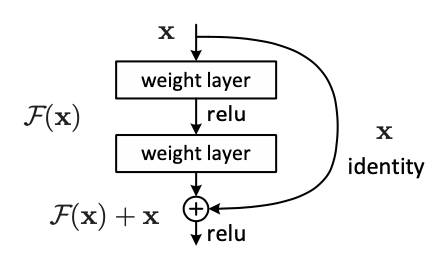
\includegraphics[width=\textwidth]{figs/residual_block.png}
		\caption{Architechture of Residual Learning\cite{resnet2016}}
		\label{fig:res}
	\end{minipage}\hfill
	\begin{minipage}{0.5\linewidth}
		\centering
		\captionof{table}{Training Condition}
		\begin{tabular}{cc}
			\toprule  % 顶部线
			Condition     & Setting   \\
			\midrule  % 中部线
			Batch Size    & 256       \\
			Epoch         & 90        \\
			Optimizer     & SGD       \\
			Learning Rate & 0.1       \\
			Momentum      & 0.9       \\
			Weight Decay  & $10^{-4}$ \\
			\bottomrule  % 底部线
		\end{tabular}
		\label{table:train_condition}
	\end{minipage}
\end{figure}


% \begin{table}[htbp]
% 	\begin{minipage}[t]{0.5\linewidth}
% 		\centering
% 		\caption{Training Condition}
% 		\begin{tabular}{cccc}
% 			\toprule  % 顶部线
% 			Condition     & Setting   \\
% 			\midrule  % 中部线
% 			Batch Size    & 256       \\
% 			Epoch         & 90        \\
% 			Optimizer     & SGD       \\
% 			Learning Rate & 0.1       \\
% 			Momentum      & 0.9       \\
% 			Weight Decay  & $10^{-4}$ \\
% 			\bottomrule  % 底部线
% 		\end{tabular}
% 	\label{table:train_condition}
% \end{minipage}
% \end{table}

By stacking different residual blocks and 1 fully connected layer, ResNet has many variants. In the experiment, we used ResNet18, ResNet50, ResNet101, ResNet152 to train and predict on our garbage dataset. The composition of these ResNet variants is show in Figure \ref{fig:res_arch}.

\begin{figure}[ht]
	\centering
	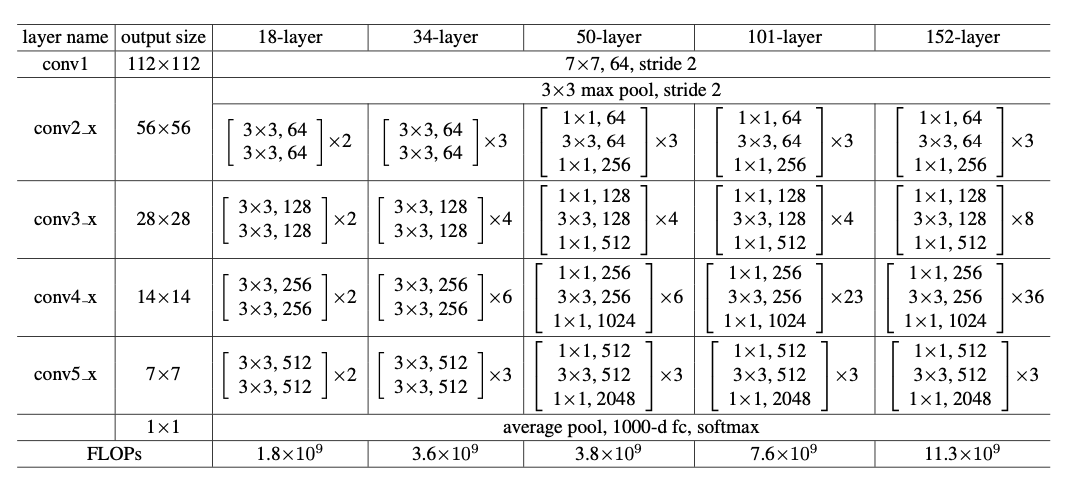
\includegraphics[width=\linewidth]{figs/resnet_arch.png}
	\caption{Architechtures of Different ResNet\cite{resnet2016}}
	\label{fig:res_arch}
\end{figure}


\subsubsection{DenseNet}
DenseNet is proposed by Gao Huang et al. \cite{densenet2017}, and won the best paper in CVPR 2017 \cite{densenet2017}. DenseNet extends the work of ResNet, building more identical shortcuts from one input to every output within the dense block. An example of a dense block with 5 convolutional layers is shown in Figure \ref{fig:dense_block}. With denser connections, DenseNet has better parameter efficiency and deeper supervision.

\begin{figure}[ht]
	\centering
	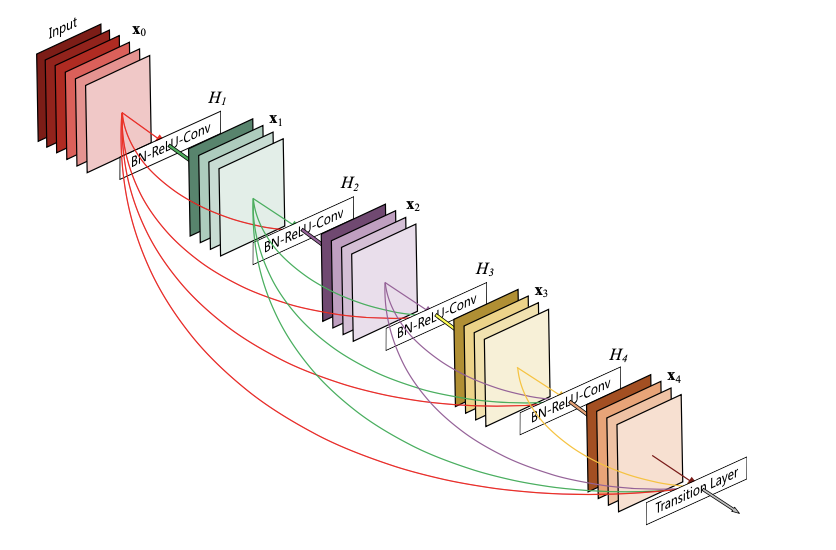
\includegraphics[width=\linewidth]{figs/dense_block.png}
	\caption{Architechtures of 5-layer Dense Block\cite{densenet2017}}
	\label{fig:dense_block}
\end{figure}

Like Resnet, the depth of DenseNet is controled by the number of stacked dense blocks. The composition of DenseNet variants is show in Figure \ref{fig:dense_arch}. In the experiment, we use DenseNet121, DenseNet161, DenseNet169 and DenseNet201 to evaluate baseline performance of DenseNet in our garbage dataset.


\begin{figure}[ht]
	\centering
	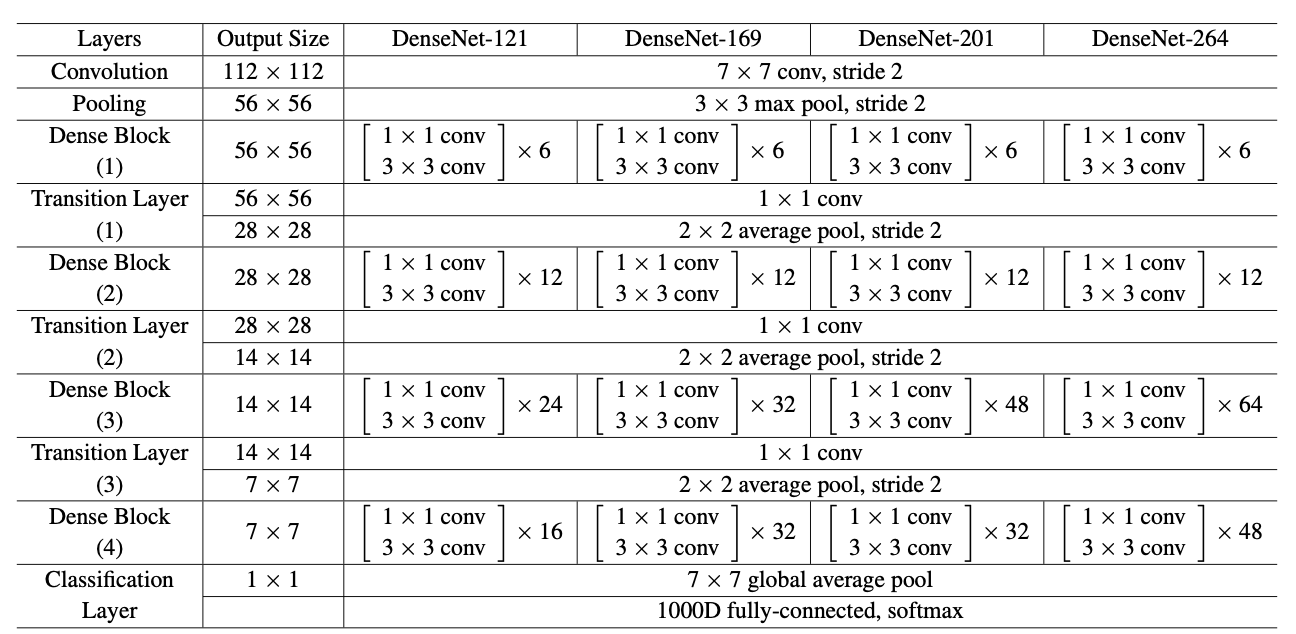
\includegraphics[width=\linewidth]{figs/dense_arch.png}
	\caption{Architechtures of DenseNet with Different Depths\cite{densenet2017}}
	\label{fig:dense_arch}
\end{figure}

\subsubsection{Experiment Setting}
We used the PyTorch version of models mentioned above, both pretrained and non-pretrained. The weights of the pretrained model have been trained on the 1000-class ImageNet dataset. We change the output channels of every model from 1000 to 42 to make the model fit to our garbage dataset. Models are trained using 10 Nvidia 2080ti GPU. Other training conditions are the same as the default settings of PyTorch official ImageNet example, which is concluded in Table \ref{table:train_condition}.

\section{Intorduction on more advanced models}
\subsection{ResNext}
ResNext is a simple, highly modularized network architecture for image classification.It is constructed
by repeating a building block that aggregates a set of transformations with the same topology. This simple design results in a homogeneous, multi-branch architecture that has only a few hyper-parameters to set. This strategy exposes a
new dimension, which is called “cardinality” (the size of the
set of transformations), as an essential factor in addition to
the dimensions of depth and width. On the ImageNet-1K
dataset, even under the restricted
condition of maintaining complexity, increasing cardinality
is able to improve classification accuracy. Moreover, increasing cardinality is more effective than going deeper or
wider when increase the capacity. ResNeXt, are the foundations of the researchers' entry to the ILSVRC
2016 classification task in which they secured 2nd place.
Further investigation shows that ResNeXt on an ImageNet-5K set and
the COCO detection set, also have better results than
its ResNet counterpart. 


\begin{figure}[H]
  \centering
  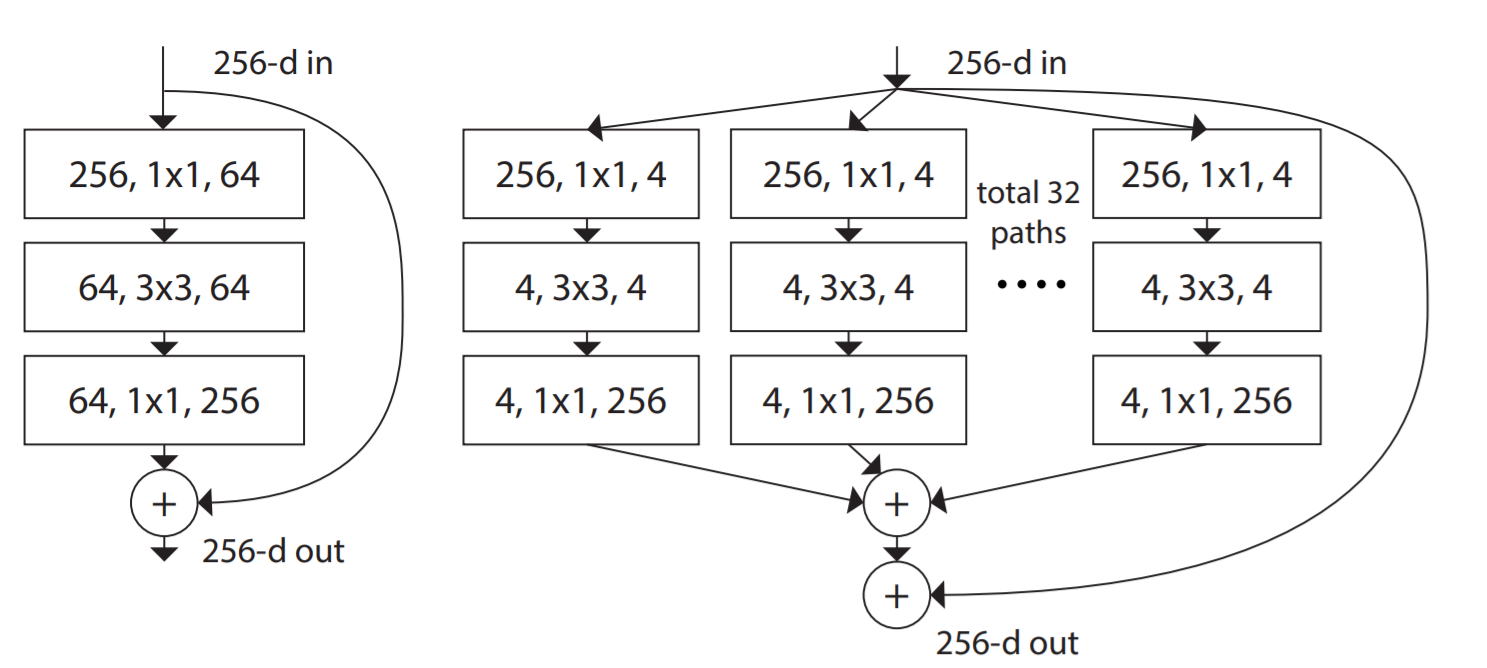
\includegraphics[width=\linewidth]{figs/cardinality.png}
  \caption{Explanation of cardinality}
  \label{fig:example}
\end{figure}
Left side is a block of ResNet. Right side is a block of
ResNeXt with cardinality = 32, with roughly the same complexity. 

With the performance of nets increase each days, human effort has been shifted to designing
better network architectures for learning representations. The VGG-nets exhibit a simple yet effective strategy of constructing very deep networks: stacking building blocks of the same shape. This strategy is inherited
by ResNets which stack modules of the same topology. This simple rule reduces the free choices of hyperparameters, and depth is exposed as an essential dimension
in neural networks. Moreover, the simplicity
of this rule may reduce the risk of over-adapting the hyperparameters to a specific dataset. The robustness of VGGnets and ResNets has been proven by various visual recognition tasks and by non-visual tasks
involving speech and language.

For the picture below,(Left) ResNet-50. (Right) ResNeXt-50 with a 32x4d
template (using the reformulation in above figure. Inside the brackets
are the shape of a residual block, and outside the brackets is the
number of stacked blocks on a stage. “C=32” suggests grouped
convolutions with 32 groups. The numbers of parameters and
FLOPs are similar between these two models.Resnext present a simple architecture which
adopts VGG/ResNets’ strategy of repeating layers, while
exploiting the split-transform-merge strategy in an easy, extensible way. A module  performs a set
of transformations, each on a low-dimensional embedding,
whose outputs are aggregated by summation.
\begin{figure}[H]
  \centering
  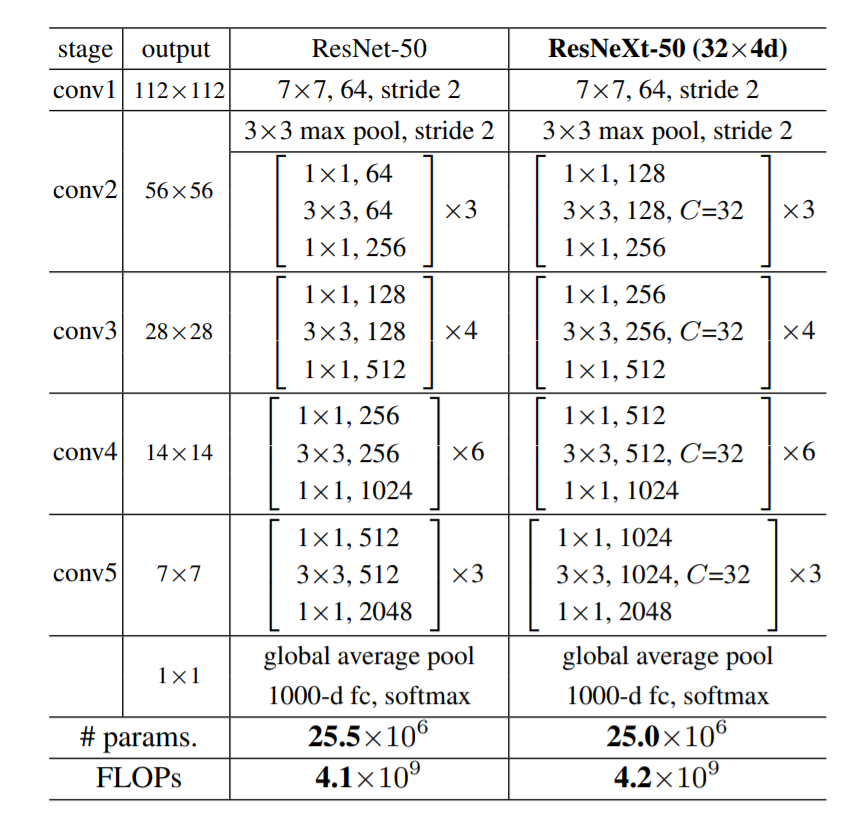
\includegraphics[width=\linewidth]{figs/structure.png}
  \caption{Structure of Resnet and Resnext}
  \label{fig:example}
\end{figure}




\begin{figure}[H]
  \centering
  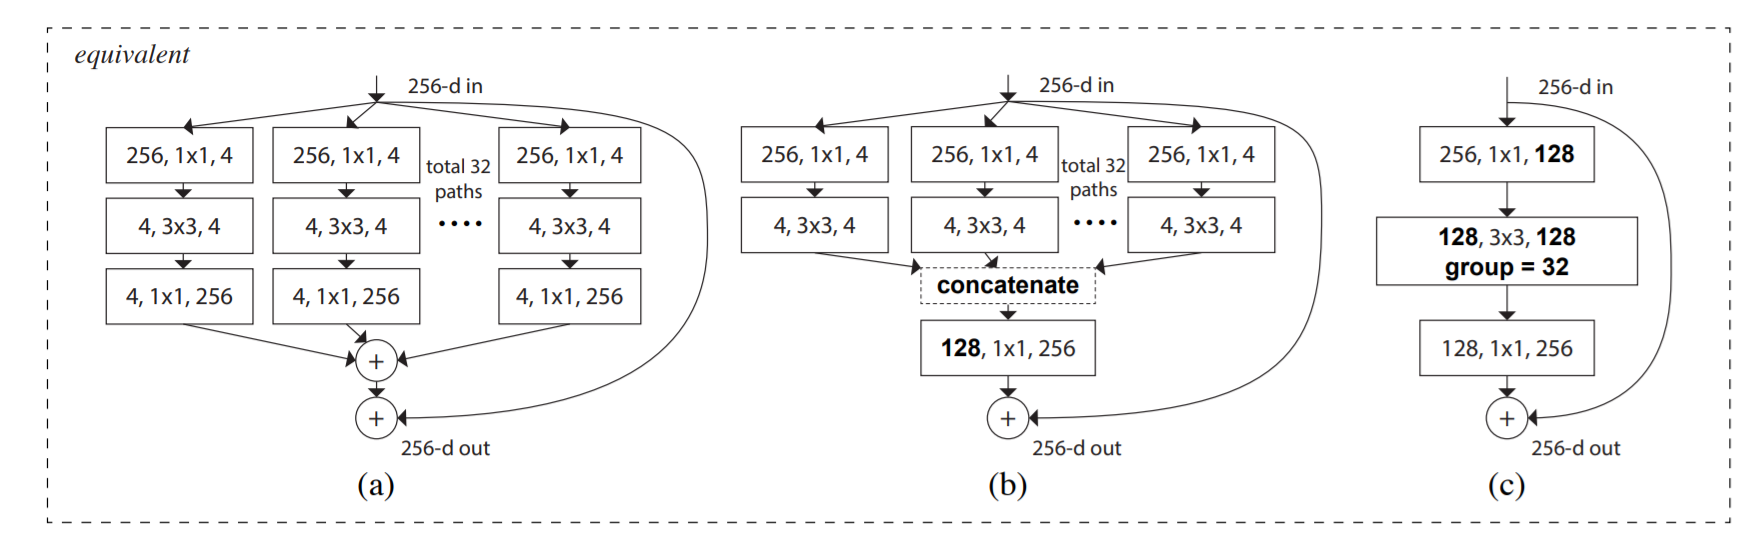
\includegraphics[width=\linewidth]{figs/equivalent.png}
  \caption{Equivalent building blocks of ResNeXt}
  \label{fig:example}
\end{figure}
(a): Aggregated residual transformations (b): A block equivalent
to (a), implemented as early concatenation. (c): A block equivalent to (a,b), implemented as grouped convolutions . Notations in bold
text highlight the reformulation changes. A layer is denoted as ( input channels, filter size,  output channels).

\subsection {fine tuning of ResNeXt}
For large-scale problems, our computation resource is always scarce. Therefore, the State-of-the-art visual perception models for a wide range of tasks rely on supervised pretraining. ImageNet classification is the classic pretraining task for these models. Yet, ImageNet is now nearly ten
years old and is by modern standards “small”. Even so, relatively little is
known about the behavior of pretraining with datasets that are multiple
orders of magnitude larger. The reasons are obvious: such datasets are
difficult to collect and annotate. Fortunately, we found a pretrained model of ResNext published by Facebook. Their dataset is obtained from tagged data on twitter. Their experiments demonstrate that training for large-scale hashtag prediction leads to excellent
results. 

\begin{figure}[H]
  \centering
  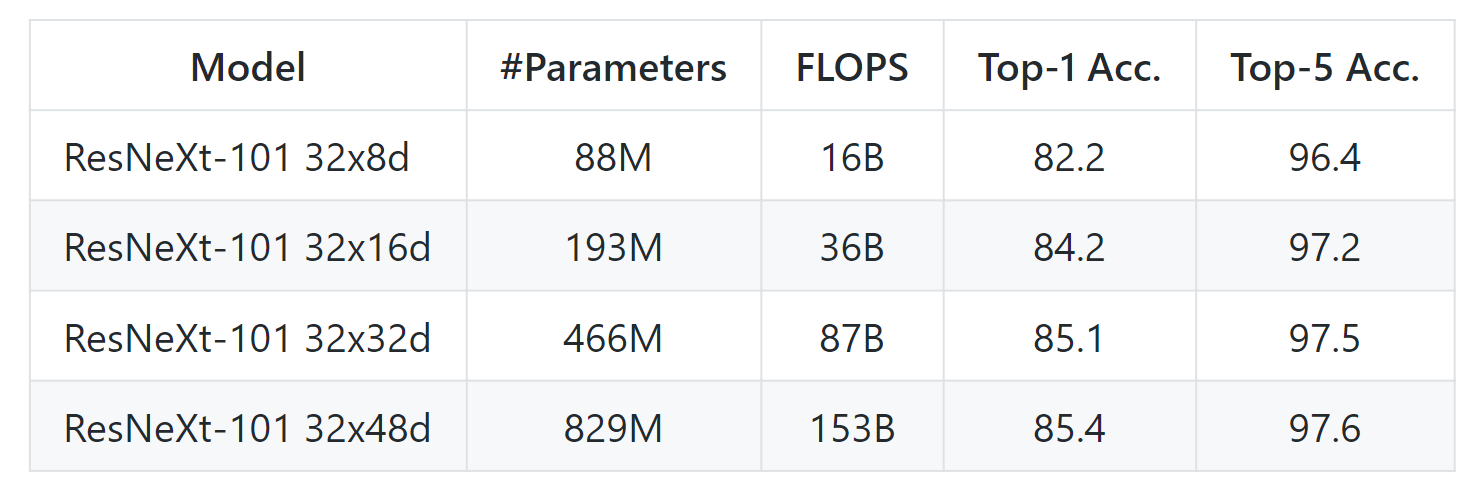
\includegraphics[width=\linewidth]{figs/pretrained-resnext.png}
  \caption{The pretrained result of resnext}
  \label{fig:example}
\end{figure}

Their models significantly improve the training accuracy on ImageNet compared to training from scratch. They achieve state-of-the-art accuracy of 85.4 on ImageNet with ResNext-101 32x48d model.


\subsection{Channel attention and spatial attention}

Attention mechanism was first proposed and used in natural language processing and machine translation aligned text, and achieved good results. In the field of computer vision, some scholars have explored the method of using attention mechanism to improve network performance in vision and convolutional neural network. The basic principle of attention mechanism is very simple: it thinks that the importance of different features (which can be different channels or different locations) in each layer of the network is different, and the latter layer should pay more attention to the important information and suppress the unimportant information. For example, in gender classification, we should pay more attention to the extraction and judgment of features that are closely related to gender, such as hair length and chest bulge, rather than the features that are not closely related to gender, such as waist thickness, height and head ratio.


When engineers and researchers design new networks, in order to improve the network capacity and performance, they usually start from three aspects: 

1. Increase the network depth: for example, from the beginning of lenet-5, to vgg-16, to resnet-101, and so on. The design of network is deeper and deeper, and the performance is better and better. When the network is deep, simply speaking, the output of the next layer is the linear combination and activation of the upper layer, which can compound more and more flexible features (in fact, it is a more complex composite function); 

2. Increase the network width: the network width here is the channel number of the feature graph. Typical examples here can range from lenet-5 to vgg-16, wider RESNET. With the increase of network width, the number of feature graph channels increases, and more convolution kernel can get more and more rich features, so the expression ability of the network is naturally strong; 

3 Enrich the network receptive field: Here we can refer to the small network composed of convolution cores with different resolutions in perception, as well as various variants in FPN and SSD. There are ways to increase the diversity of receptive field to improve performance. Different receptive fields have different ability of feature extraction and expression for different sizes of objects. Generally, the pixels with large receptive field on the feature map can better represent the information extracted from the large objects, while the pixels with small receptive field can only see a part of the large objects. Conversely, the pixels with large receptive field can see too much field of vision, and there is too much redundant information and information for small objects Noise. Therefore, the use of different resolution receptive field, rich network receptive field to improve the network, let the big receptive field to deal with the big goal, small receptive field to deal with the small goal, each perform their own duties, to improve the network performance has become a lot of natural means of network design. 

\begin{figure}[H]
  \centering
  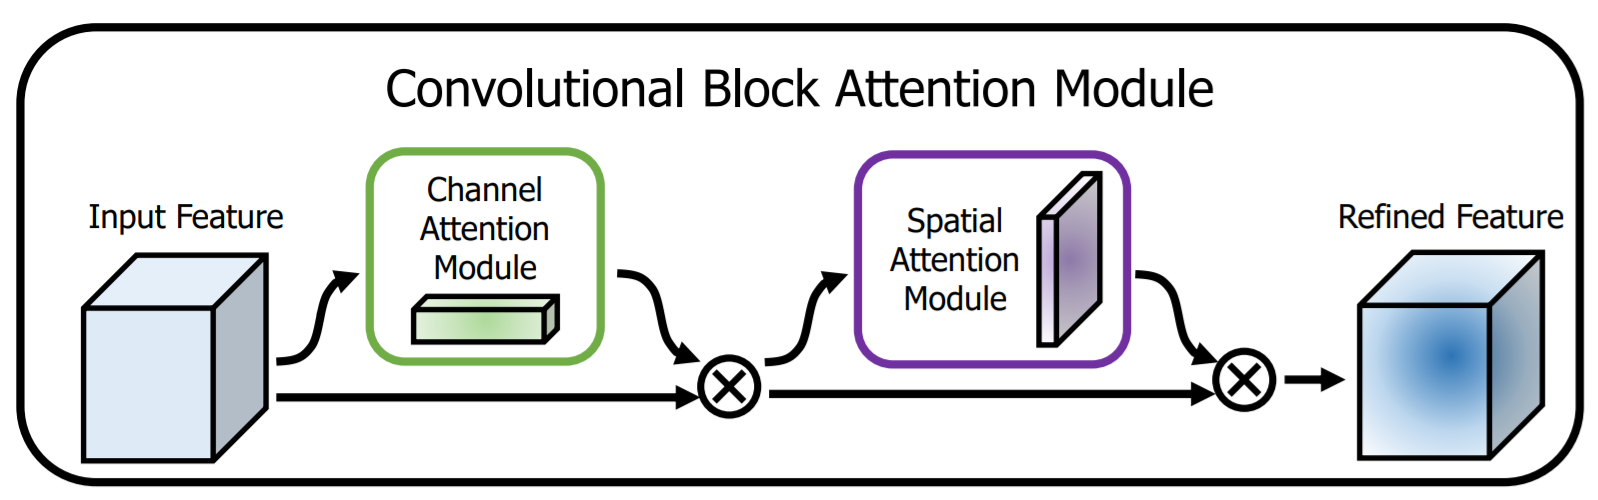
\includegraphics[width=\linewidth]{figs/attention1.png}
  \caption{Convolutional Block Attention Module}
  \label{fig:example}
\end{figure}

Above is the overview of CBAM. The module has two sequential sub-modules:
channel and spatial. The intermediate feature map is adaptively refined through
our module (CBAM) at every convolutional block of deep networks.

\begin{figure}[H]
  \centering
  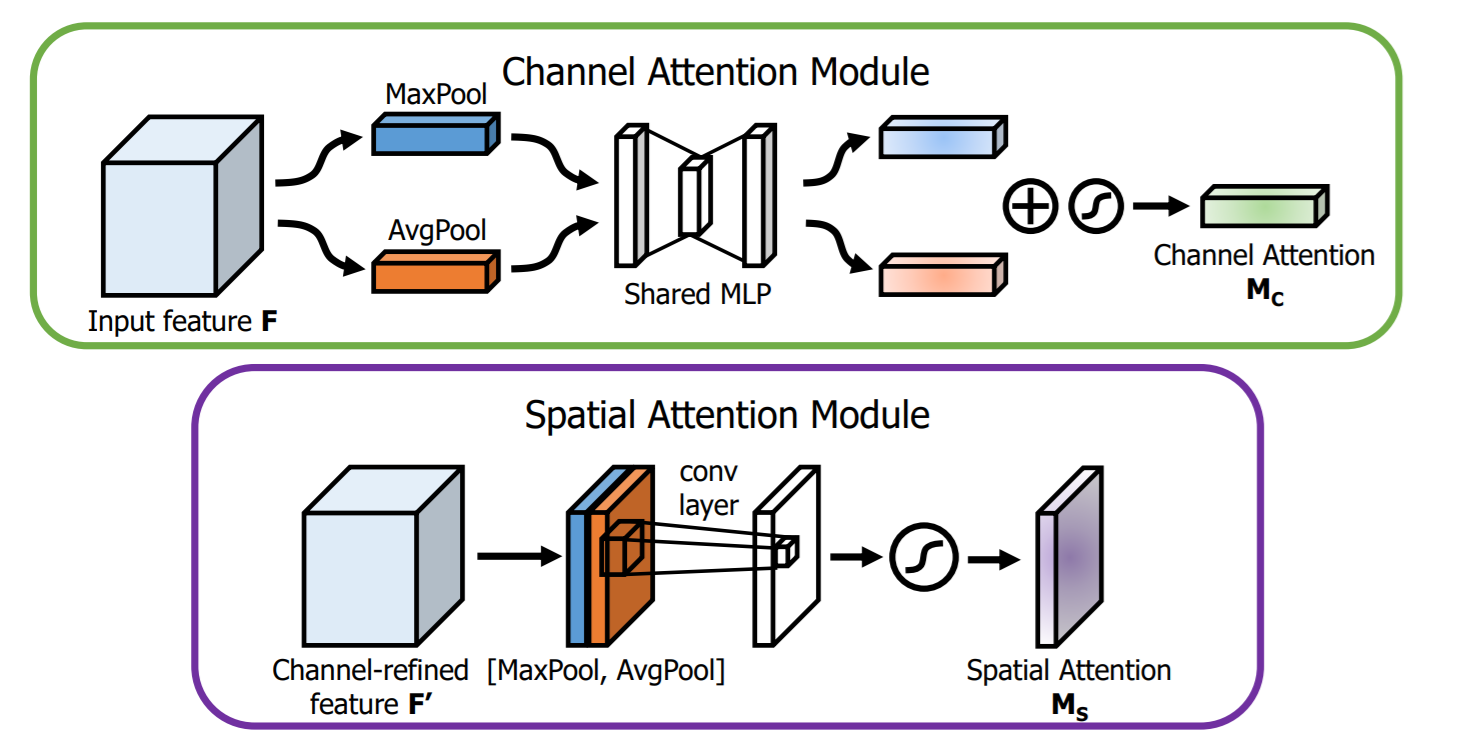
\includegraphics[width=\linewidth]{figs/cansam.png}
  \caption{Convolutional Block Attention Module and Spatial attention Module}
  \label{fig:example}
\end{figure}

Above is diagram of each attention sub-module. As illustrated, the channel
sub-module utilizes both max-pooling outputs and average-pooling outputs with
a shared network; the spatial sub-module utilizes similar two outputs that are
pooled along the channel axis and forward them to a convolution layer.

Of course, many network designs also consider the combination of these three for more elaborate design, and the essence of the idea is the same. CBAM is different from the three ideas mentioned above. It does not increase the depth of the network, the width of the network, or the convolution kernel of different kernel sizes. It adjusts the existing feature maps selectively and more precisely To improve the performance of the network.


\begin{figure}[H]
  \centering
  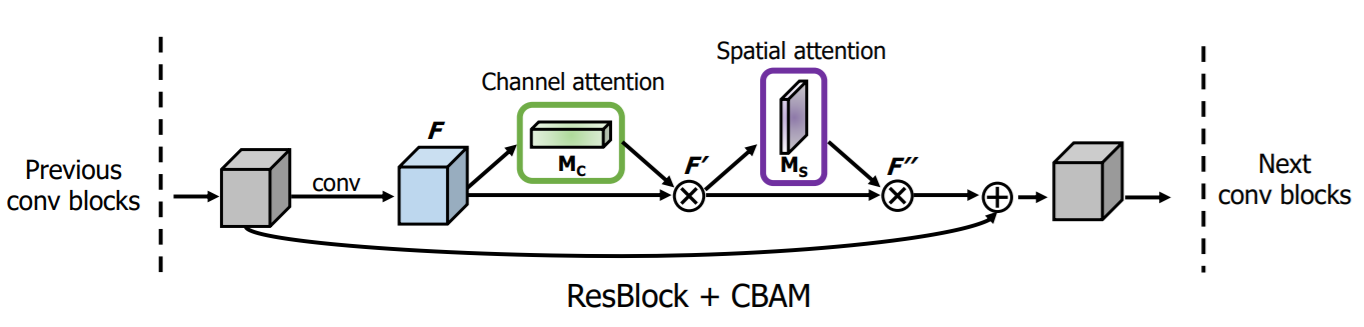
\includegraphics[width=\linewidth]{figs/cares.png}
  \caption{CBAM integrated with a ResBlock in ResNet}
  \label{fig:example}
\end{figure}

This figure shows
the exact position of our module when integrated within a ResBlock. CBAM is applied on the convolution outputs in each block.

As for the spatial attention, we can see below:

\begin{figure}[H]
  \centering
  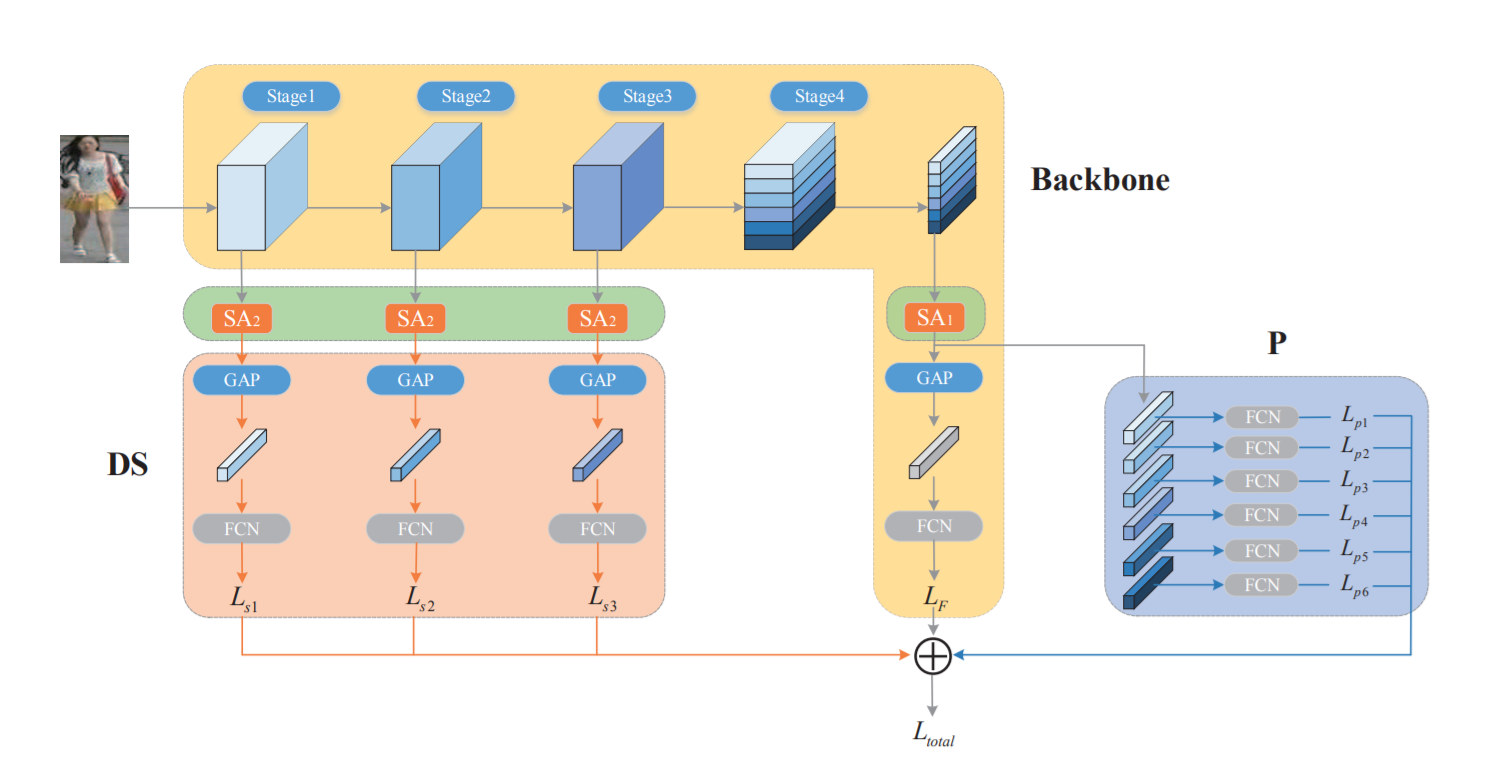
\includegraphics[width=\linewidth]{figs/spatial1.png}
  \caption{spatial attention}
  \label{fig:example}
\end{figure}

The proposed architecture formulates the task as a classification. It consists of four components. The yellow region represents the
backbone feature extractor. The red region represents the deeply supervised branches (DS). The blue region represents six part classifiers
(P) . The two green region represents two sets of spatial attention layers (SA), SA1 is not used for the main results. Then the total loss is the summation over all deep supervision losses, six part losses and the
loss from the backbone. Note that the spatial attention is only added before GAP.

\begin{figure}[H]
  \centering
  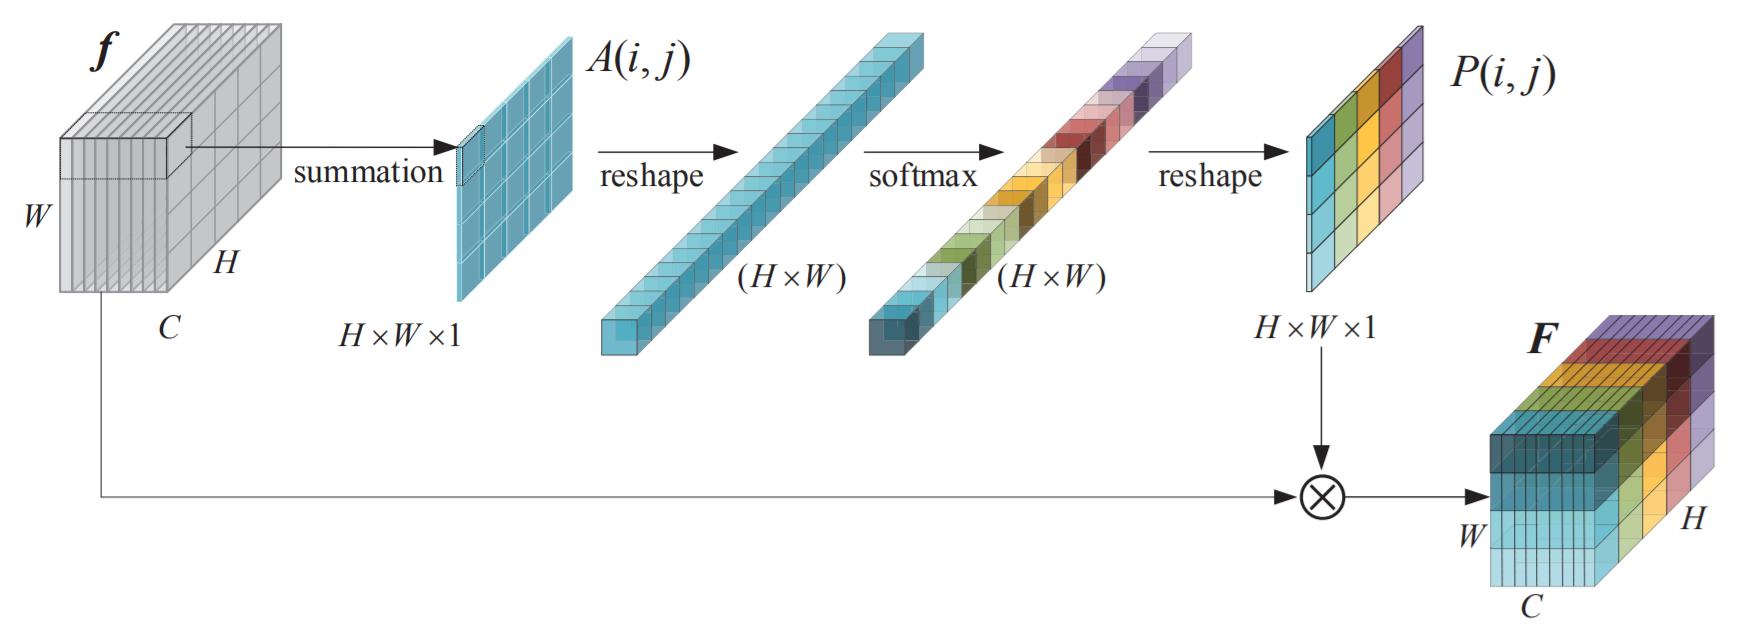
\includegraphics[width=\linewidth]{figs/spatial2.png}
  \caption{Spatial attention}
  \label{fig:example}
\end{figure}

Parameter-free spatial attention layer has no trainable parameter. It assigns different importance for different locations. It consists
of a summation and a softmax. A(i, j) denotes the summation over the activations along the channel. The softmax values are computed over A then multiplied to all activations from the same location.

\subsection{Top Advanced model}
Our final model is based on the runner-up's published code. It contains channel attention and spatial attention. We also performed some techniques on the model. Include: data augmentation, test time augmentation and different optimizers and learning schdulers. The training enviroment is an existing server in our lab. The major training process is runned on a server with 6 2080Ti GPUs avaliable.  Due to the complexity of structure and modules and also the limit of time, we preserve the net's structure  which is the ResNext with spatial and channel attention. One epoch usually takes about 10 minutes including training and evaluating time. As for 50 epochs, it takes one night.

\subsection{Data Augmentation and Fine tuning}
We applied several trasformation methods on the data. Including centercrops,randomcrops, randomearase, random horizontal flip, ramdom rotation and brightness adjustment.

We choose a composition with good performance in the code, but there is no gurantee it is the best. Indeed, data augmentation methods is effective in generalization, but not that much. We think although the dataset cannot compare to some famous big set but it is relatively big. So data augmentation is not desperate. The improvement is around 1 percent in different settings.

As for the test time augmentation, it is arguablely cheating method. We implement it but not used it in the final evaluation. The test accuracy could raise about 1.5 percent.

The learning parameters and the schedule is also adjusted. The learning parameters with in the resnext is 0.001 and the last fully connected layer is 0.01. The learning rate multiplies by 0.5 every 8 epochs.

Within 10 epoch, the model always reach a very high accuracy on the training set, higher than 99.5 percents. But the validation accuracy is always around 93 percents, which indicates there is severe over-fitting. Unfortunately, we tried our best in overcame this, but the result is not that good. Apart from almost all the preprocessing  methods, we tried to tune the dropout parameter, but the effect is subtle.

\subsection{Heatmaps of class activation}

This general category of techniques is called class activation map (CAM) visualization,
and it consists of producing heatmaps of class activation over input images. A class activation heatmap is a 2D grid of scores associated with a specific output class, computed
for every location in any input image, indicating how important each location is with respect to the class under consideration. For instance, given an image fed into a dogsversus-cats convnet, CAM visualization allows you to generate a heatmap for the class
“cat,” indicating how cat-like different parts of the image are, and also a heatmap for the
class “dog,” indicating how dog-like parts of the image are.
 
it consists of taking the output feature map of a convolution layer, given an input
image, and weighing every channel in that feature map by the gradient of the class
with respect to the channel. Intuitively, one way to understand this trick is that we’re
weighting a spatial map of “how intensely the input image activates different channels” by “how important each channel is with regard to the class,” resulting in a spatial
map of “how intensely the input image activates the class.”

\begin{figure}[H]
  \centering
  \includegraphics[width=\linewidth]{figs/OIP.jpg}
  \caption{Class activation Map}
  \label{fig:example}
\end{figure}

We can see from the heatmaps below ,what the neural net learns and cares most in the image, and rely more on this area to make the right decision.

\begin{figure}[H]

  \begin{minipage}[t]{.3\linewidth}
    \centering
    \includegraphics[width=\textwidth]{figs/0cam.jpg}
    
  \end{minipage}
  \hfill
\begin{minipage}[t]{.3\linewidth}
    \centering
    \includegraphics[width=\textwidth]{figs/1cam.jpg}
    
  \end{minipage}
  \hfill
  \begin{minipage}[t]{.3\linewidth}
    \centering
    \includegraphics[width=\textwidth]{figs/2cam.jpg}
    
  \end{minipage}
  \hfill
  \begin{minipage}[t]{.3\linewidth}
    \centering
    \includegraphics[width=\textwidth]{figs/3cam.jpg}
    
  \end{minipage}
  \hfill
  \begin{minipage}[t]{.3\linewidth}
    \centering
    \includegraphics[width=\textwidth]{figs/4cam.jpg}
    
  \end{minipage}
  \hfill
\begin{minipage}[t]{.3\linewidth}
    \centering
    \includegraphics[width=\textwidth]{figs/5cam.jpg}
   
  \end{minipage}
  \hfill
\begin{minipage}[t]{.3\linewidth}
    \centering
    \includegraphics[width=\textwidth]{figs/6cam.jpg}
    
  \end{minipage}
  \hfill
\begin{minipage}[t]{.3\linewidth}
    \centering
    \includegraphics[width=\textwidth]{figs/7cam.jpg}
    
  \end{minipage}
  \hfill
  \begin{minipage}[t]{.3\linewidth}
    \centering
    \includegraphics[width=\textwidth]{figs/8cam.jpg}
    
  \end{minipage}
  \hfill
\begin{minipage}[t]{.3\linewidth}
    \centering
    \includegraphics[width=\textwidth]{figs/9cam.jpg}
    
  \end{minipage}
  \hfill
\begin{minipage}[t]{.3\linewidth}
    \centering
    \includegraphics[width=\textwidth]{figs/10cam.jpg}
    
  \end{minipage}
  \hfill
  \begin{minipage}[t]{.3\linewidth}
    \centering
    \includegraphics[width=\textwidth]{figs/11cam.jpg}
    
  \end{minipage}
  \hfill
  \caption{Heatmaps of class activation}
  \vspace{-3mm}
  
\end{figure}



\begin{figure}[H]

  \begin{minipage}[t]{.3\linewidth}
    \centering
    \includegraphics[width=\textwidth]{figs/12cam.jpg}
    
  \end{minipage}
  \hfill
\begin{minipage}[t]{.3\linewidth}
    \centering
    \includegraphics[width=\textwidth]{figs/13cam.jpg}
    
  \end{minipage}
  \hfill
  \begin{minipage}[t]{.3\linewidth}
    \centering
    \includegraphics[width=\textwidth]{figs/14cam.jpg}
    
  \end{minipage}
  \hfill
  \begin{minipage}[t]{.3\linewidth}
    \centering
    \includegraphics[width=\textwidth]{figs/15cam.jpg}
    
  \end{minipage}
  \hfill
  \begin{minipage}[t]{.3\linewidth}
    \centering
    \includegraphics[width=\textwidth]{figs/16cam.jpg}
    
  \end{minipage}
  \hfill
\begin{minipage}[t]{.3\linewidth}
    \centering
    \includegraphics[width=\textwidth]{figs/17cam.jpg}
   
  \end{minipage}
  \hfill
\begin{minipage}[t]{.3\linewidth}
    \centering
    \includegraphics[width=\textwidth]{figs/18cam.jpg}
    
  \end{minipage}
  \hfill
\begin{minipage}[t]{.3\linewidth}
    \centering
    \includegraphics[width=\textwidth]{figs/19cam.jpg}
    
  \end{minipage}
  \hfill
  \begin{minipage}[t]{.3\linewidth}
    \centering
    \includegraphics[width=\textwidth]{figs/20cam.jpg}
    
  \end{minipage}
  \hfill
\begin{minipage}[t]{.3\linewidth}
    \centering
    \includegraphics[width=\textwidth]{figs/21cam.jpg}
    
  \end{minipage}
  \hfill
\begin{minipage}[t]{.3\linewidth}
    \centering
    \includegraphics[width=\textwidth]{figs/22cam.jpg}
    
  \end{minipage}
  \hfill
  \begin{minipage}[t]{.3\linewidth}
    \centering
    \includegraphics[width=\textwidth]{figs/23cam.jpg}
    
  \end{minipage}
  \hfill
  \caption{Heatmaps of class activation}
  \vspace{-3mm}
  
\end{figure}

\begin{figure}[H]

  \begin{minipage}[t]{.3\linewidth}
    \centering
    \includegraphics[width=\textwidth]{figs/24cam.jpg}
    
  \end{minipage}
  \hfill
\begin{minipage}[t]{.3\linewidth}
    \centering
    \includegraphics[width=\textwidth]{figs/25cam.jpg}
    
  \end{minipage}
  \hfill
  \begin{minipage}[t]{.3\linewidth}
    \centering
    \includegraphics[width=\textwidth]{figs/26cam.jpg}
    
  \end{minipage}
  \hfill
  \begin{minipage}[t]{.3\linewidth}
    \centering
    \includegraphics[width=\textwidth]{figs/27cam.jpg}
    
  \end{minipage}
  \hfill
  \begin{minipage}[t]{.3\linewidth}
    \centering
    \includegraphics[width=\textwidth]{figs/28cam.jpg}
    
  \end{minipage}
  \hfill
\begin{minipage}[t]{.3\linewidth}
    \centering
    \includegraphics[width=\textwidth]{figs/29cam.jpg}
   
  \end{minipage}
  \hfill
\begin{minipage}[t]{.3\linewidth}
    \centering
    \includegraphics[width=\textwidth]{figs/30cam.jpg}
    
  \end{minipage}
  \hfill
\begin{minipage}[t]{.3\linewidth}
    \centering
    \includegraphics[width=\textwidth]{figs/31cam.jpg}
    
  \end{minipage}
  \hfill
  \begin{minipage}[t]{.3\linewidth}
    \centering
    \includegraphics[width=\textwidth]{figs/32cam.jpg}
    
  \end{minipage}
  \hfill

  \caption{Heatmaps of class activation}
  \vspace{-3mm}
  
\end{figure}
\begin{figure}[H]
\begin{minipage}[t]{.3\linewidth}
    \centering
    \includegraphics[width=\textwidth]{figs/33cam.jpg}
    
  \end{minipage}
  \hfill
\begin{minipage}[t]{.3\linewidth}
    \centering
    \includegraphics[width=\textwidth]{figs/34cam.jpg}
    
  \end{minipage}
  \hfill
  \begin{minipage}[t]{.3\linewidth}
    \centering
    \includegraphics[width=\textwidth]{figs/35cam.jpg}
    
  \end{minipage}
  \hfill
  \begin{minipage}[t]{.3\linewidth}
    \centering
    \includegraphics[width=\textwidth]{figs/36cam.jpg}
    
  \end{minipage}
  \hfill
\begin{minipage}[t]{.3\linewidth}
    \centering
    \includegraphics[width=\textwidth]{figs/37cam.jpg}
    
  \end{minipage}
  \hfill
  \begin{minipage}[t]{.3\linewidth}
    \centering
    \includegraphics[width=\textwidth]{figs/38cam.jpg}
    
  \end{minipage}
  \hfill
  \begin{minipage}[t]{.3\linewidth}
    \centering
    \includegraphics[width=\textwidth]{figs/39cam.jpg}
    
  \end{minipage}
  \hfill
  \begin{minipage}[t]{.3\linewidth}
    \centering
    \includegraphics[width=\textwidth]{figs/40cam.jpg}
    
  \end{minipage}
  \hfill
\begin{minipage}[t]{.3\linewidth}
    \centering
    \includegraphics[width=\textwidth]{figs/41cam.jpg}
   
  \end{minipage}
  \hfill

  \caption{Heatmaps of class activation}
  \vspace{-3mm}
  
\end{figure}

The examples of heatmaps are randomly chosen. We can tell that for most of the cases it learns the most important feature of the image. Like the pull ring of a can, or ash and smoke of cigrattes. But sometimes it may put wrong attention. Like the aspirin pill case, the net focus most on the line on the packing.